%
% The 'sig-alternate.cls'-V2.5 LaTeX2e document class file has been used to 
% generate this document so that it complies with the ACM article submission 
% standard for Conference 
%
% Author

\documentclass{sig-alternate-05-2015}

\newcommand{\univ} {Michigan Technological University}
\newcommand{\addra}{1400 Townsend Dr.}
\newcommand{\addrb}{Houghton, MI 49931}
\renewcommand{\email}{\normalsize{}}

\begin{document}

% Copyright
%\setcopyright{acmcopyright}

% Title
\title{Smart Farming via. Distributed Sensing}

%
% Author's
\numberofauthors{5}
\author{
% 1st. author
\alignauthor
Akhil Kurup\\
       \affaddr{\univ}\\
       %\affaddr{\addra}\\
       %\affaddr{\addrb}\\
       \email{amkurup@mtu.edu}
% 2nd. author
\alignauthor
Krishna Karan Kumar\\
       \affaddr{\univ}\\
       %\affaddr{\addra}\\
       %\affaddr{\addrb}\\
       \email{menduk@mtu.edu}
% 3rd. author
\alignauthor 
Ravikumar Chilmula\\
       \affaddr{\univ}\\
       %\affaddr{\addra}\\
       %\affaddr{\addrb}\\
       \email{rchilmul@mtu.edu}
\and   % use '\and' if you need 'another row' of author names
% 4th. author
\alignauthor 
Sarala Ravindra\\
       \affaddr{\univ}\\
       %\affaddr{\addra}\\
       %\affaddr{\addrb}\\
       \email{sravindr@mtu.edu}
% 5th. author
\alignauthor 
Prof. Zhaohui Wang\\
       \affaddr{\univ}\\
       %\affaddr{\addra}\\
       %\affaddr{\addrb}\\
       \email{zhaohuiw@mtu.edu}
} % End author list

%
\maketitle
%

\begin{abstract}
Agriculture produce of the world should meet the rate of population growth in order to be able to feed everyone. The Food and Agriculture organization (FAO) predicts that the current rate of agriculture produce should be increased by almost 70\% by 2050. However, on the contrary, the recent produce has declined due to limited availability of man-power, land and water resources and climate change. A deviation from traditional methods is necessary to meet the need of the growing population. At such a juncture, automating the process of farming seems to be the way to go. Previous works towards this effort have been proven to be effective. However their cost and complexity prevents their use on a large scale. This article discusses the authors plan to integrate electronics with traditional farming practices. The use of sensors for land and water management and food safety has been demonstrated and some of the results have also been included.
\end{abstract}


\keywords{Smart Farming, Embedded Sensor Networks, Telos-B, TinyOS, Raspberry-Pi, OpenCV, Localization}


\section{Introduction}
The Food and Agriculture organization (FAO) of the United Nations predicts that the population growth by 2050 would be in the vicinity of 9.6 billion people\cite{fao:fao1}. To feed this entire population, the food production must increase by 70\%\cite{fao:fao1}. Conventional farming has become stagnant due to the limited availability of usable water and land resources. Moreover, modernization has seen a steady decline in the number of farmers over the years. In recent years climate change is also posing to be a potential threat by indirectly affecting the crop yield. The FAO therefore recommends the use of modern techniques, namely digital tools, to increase the agriculture yield and meet the growing needs of the future.

Several areas of farming can be improved using modern techniques like management of farm vehicles, livestock monitoring, storage and inventory management and arable farming. The authors are concentrating their efforts towards arable agriculture specifically water management. 
Smart farming is the use of electronics, control  systems  and information technology systems to  optimize productivity and  delivery  of  crop produce. The available technologies in smart farming are either too futuristic and not deploy able or are available to only few of the large farms.

The modern growth in Internet of Things (IoT) can be applied towards increasing the produce of crops\cite{bcm:bcm1}. The authors hope to integrate this well known electronics to form localized sensor networks to precisely collect and process data and relay the information to the user. This would reduce the manpower required and the processed data will supplement for the skilled workers. The authors aim towards demonstrating embedded network formation and its implementation towards this real life problem and hope to stress on the impact of technology in our lives.

Gathering data is of utmost importance and forms a building block that influences smart farming. Historical data such as weather events, climate, economics, machine settings, etc. are all useful data that would aid the decision making of farmers. Several data sources can be present that involve but not limited to satellite imagery, aerial surveillance (using drones) and land based measurements (both manual as well as automated). The authors target small farms and keeping cost in mind have opted for small and relatively inexpensive embedded platforms that also do not require much expertise to operate.
In the long run, data from several farms can be collected and processed to further learn patterns in crop produce. Big data analysis and pattern recognition techniques including deep learning can be applied to better understand the phenomenon. The results can be uploaded into the devices to help farmers make precise decisions on the fly.

The authors are in the process of developing a system that can be deployed on a field to help reduce the manual efforts required in farming and at the same time maximize the yield of crops. They have developed embedded solutions based on popular hardware and software platforms and plan to use image processing techniques towards realizing their concept. The further sections describe the concept used by the authors and give details on their implementation and some intricacies involved in their system design.


\section{System Components}
Embedded systems are an integral part of our day to day activities. They are present in cell-phones, cars, TVs, heating systems, etc. They are one of most rapidly growing segments in the industry. It is only natural that the authors have decided to apply embedded systems to their application. The current application has been designed to operate standalone in the field. This requires an intricate balance between the underlying hardware platform and the software that should run on this platform. This section describes the various components that build the system in brief.\\

\subsection{Hardware}
Embedded hardware should have \textit{low power consumption}, \textit{small form factor} and \textit{low cost}. With such considerations, choice of the hardware varies greatly from application to application. This subsection describes the hardware chosen by the authors and some of their features.\\

The \textit{Telos-B mote (TPR2420)} is a wireless embedded sensor that has been used as a node in several applications. Its small form factor, easy availability, cost and available development platforms make it a very desirable choice for many applications. The availability of on-board sensors such as moisture and temperature sensors can be directly used in the current application. Figure \ref{TelosB} shows the various blocks available on a conventional off-the-shelf TPR2420 sensor node.
\begin{figure}[h]
\centering
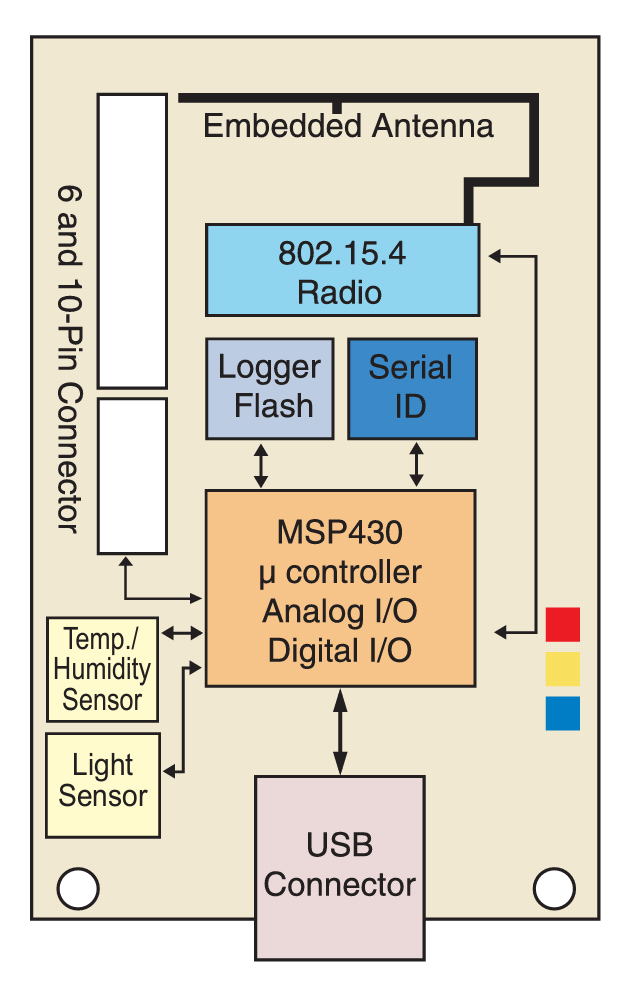
\includegraphics[width=1.5in]{TelosB.png}
\caption{Block level representation showing the components on a Telos-B (TPR2420)}
\label{TelosB}
\end{figure}

Some of it's key features of the are:
\begin{enumerate}
\item 8 MHz TI MSP430 micro-controller with 10kB RAM
\item IEEE 802.15.4/ZigBee compliant RF transceiver 
\item 2.4 to 2.4835 GHz, a globally compatible ISM band
\item 250 kbps data rate
\item Programming and data collection via USB
\item Integrated light, temperature and humidity sensor
\item Supported by TinyOS 1.1.10 and higher
\end{enumerate}

The \textit{Raspberry-Pi} is a single board computer developed by the Raspberry Pi foundation. It houses a powerful Processor with limited RAM and can host popular Linux distros. namely Raspbian and Ubuntu. Figure \ref{rpi} shows a RPi ModelB+, similar to the one the authors have proposed to use in their application.
Some of the impressive features are:
\begin{enumerate}
\item 900MHz quad-core ARM Cortex-A7 CPU
\item 1GB RAM
\item Micro SD card slot
\item VideoCore-IV 3D graphics core
\item 4 USB ports
\end{enumerate}

\begin{figure}[hbtp]
\centering
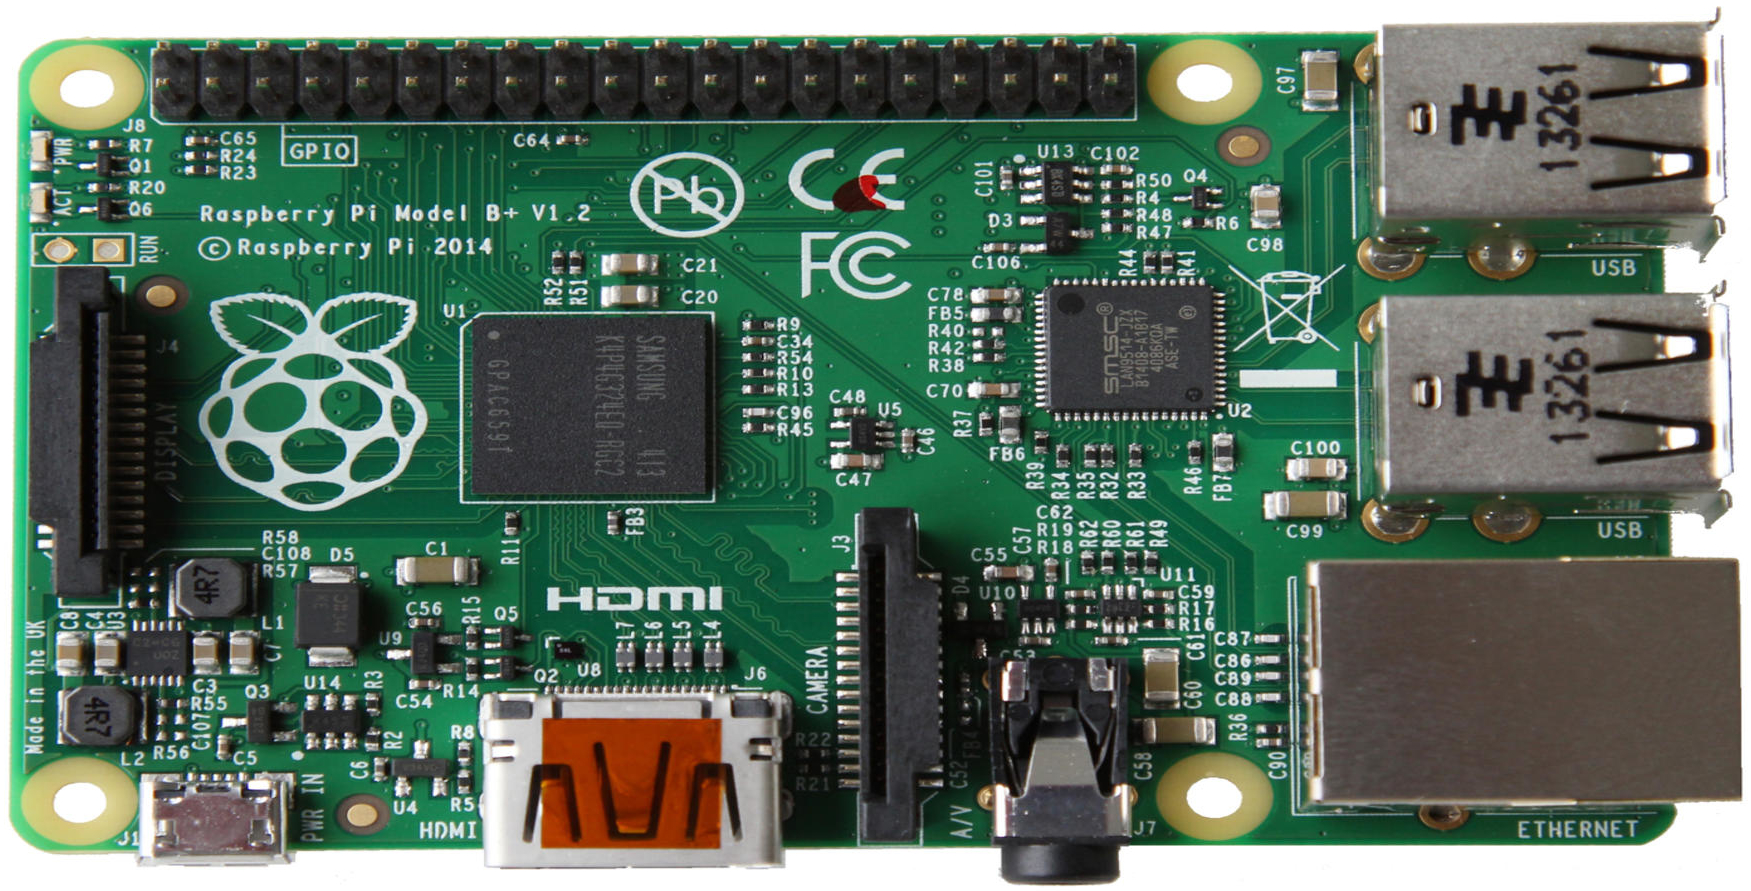
\includegraphics[height=1.75in, width=2.5in]{RPi2.jpg}
\caption{The popular Raspberry Pi single-board computer}
\label{rpi}
\end{figure}

\subsection{Software}
This section describes the software components used in our project. This software goes hand-in-hand with the hardware to deploy our application.\\

The open-source \textit{TinyOS}\cite{tinyos:tinyos} distribution provides full support for the Telos-B mote. It has been designed and optimized for low-power wireless embedded sensors. It includes a strong work scheduler and an optimized collection of drivers that support a hoard of common micro-controllers and sensor modules. TinyOS supports programs written in nesC\cite{nesc:nesc} which is an extension to the widely popular \texttt{C} programming language designed to embody the structuring concepts and execution model of TinyOS. Another feature that greatly benefits the use of TinyOS on embedded platforms is its inherent \textit{event-driven} nature. Installation and usage of TinyOS can be done through any Linux distro. XubunTOS includes a set of prerequisite binaries and native support to run the TinyOS on the TelosB mote.

OpenCV is the preferred software for image processing. It was developed by Intel\cite{intel:intel} and is distributed as an open BSD package. It can run on both C++ as well as Python making it extremely robust and portable across platforms. 

\section{Proposed Implementation}
Towards Smart Farming, the authors have proposed to use the popular \textit{TelosB}\cite{telosb:telosb} motes in conjunction with a \textit{Raspberry-Pi}\cite{rpi:rpi2}. Figure \ref{smart} shows a diagrammatic representation of the authors plan to implement smart farming. One of the glitches the authors faced was communication between the Telos-B and the Raspberry-Pi. To circumvent this, one TelosB was used as a data communication gateway between the other nodes and the Raspberry-Pi over the USB. The communication between the Telos-B-HUB and other nodes is done over the IEEE 802.15.4\cite{zigbee:zigbee} protocol.

\begin{figure}[h]
\centering
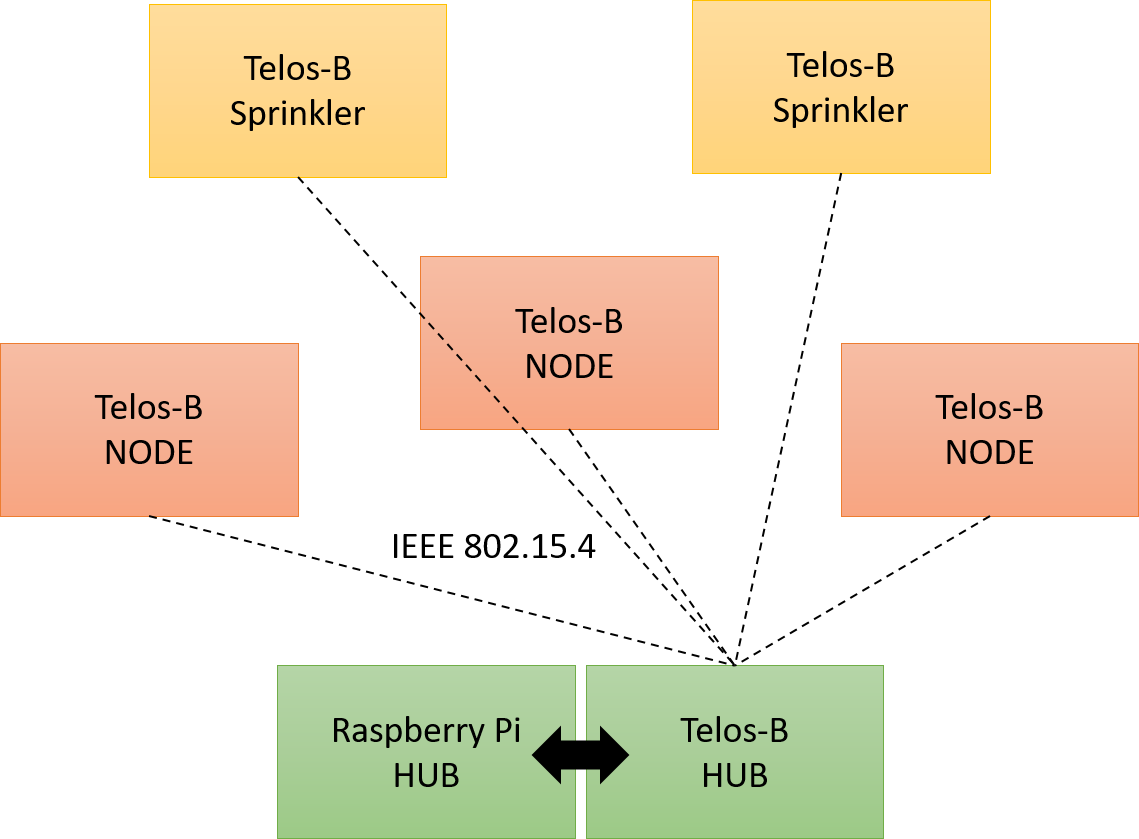
\includegraphics[width=3.2in]{sys.png}
\caption{Block level representation showing the various components involved in the smart farming system}
\label{smart}
\end{figure}

Initially the Raspberry-Pi will be mounted on a small rover-like robot and traversed through the field. A web-cam would be connected to the Raspberry-Pi on its USB port which would keep clicking photos of its surrounding at every 1-second interval as shown in Figure \ref{rpi2}. After the complete field has been traversed, all the images would be assimilated and stitched together to create a "map" of the field. The TelosB Nodes will then be mounted on a small rover-like robot and traversed through the field. At each point they will check for the moisture and temperature of the soil and dynamically make a decision of the condition of the soil. 
\begin{figure}[h]
\centering
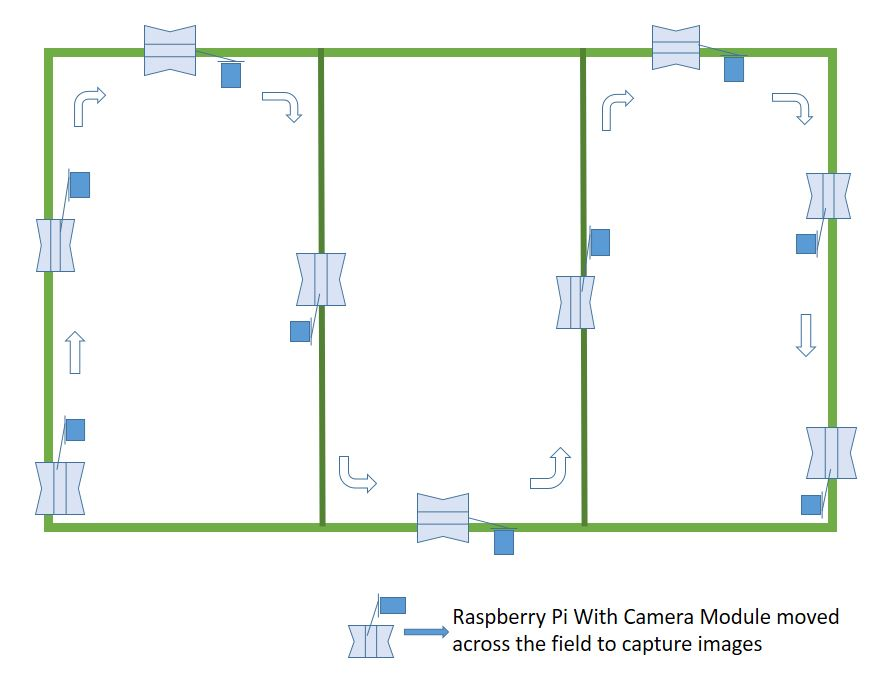
\includegraphics[width=3.2in]{RPi_imgs.jpg}
\caption{Initial traversal of the Raspberry-Pi HUB across the field to take pictures and create a database of images}
\label{rpi2}
\end{figure}
If the water content is found to be less, the position of the node is noted (as described in the further sections) and the traversal continues. Sprinklers are connected to the TelosB motes (called TelosB sprinklers) via solenoids that can be controlled by simple TTL signals from the mote. Once the decision has been made, the TelosB-sprinklers are enabled by the HUB to start the watering process. Depending on the condition of the soil, the amount of water is regulated.

Figure \ref{flow} shows a block level representation of the flow of data between the different blocks. This is a very primitive representation.

\begin{figure}[h]
\centering
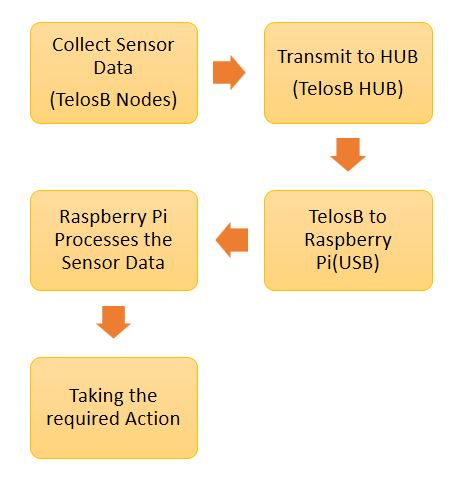
\includegraphics[width=2.3in]{flow.jpg}
\caption{Showing the flow of control and data between the various components}
\label{flow}
\end{figure}


\subsection{Localization}
Localization in an wireless network is the process of finding the position of a node within a network. Often data has little value if the position information is not available. Arguably, the most popular Global Positioning System (GPS) comes at a price in terms of power and radio resources. Anchor based, anchor free, centralized and distributed localization are the popular methods used in embedded systems due to their relative low resource requirements. Range free and range based techniques could be \textit{anchor-based} which assume the presence of sensor nodes in the network that have knowledge about their location or \textit{anchor-free} which estimate relative positions of nodes instead of computing absolute node positions.

Range based techniques depends on estimation of either angle or distance or both of an un-localized node with respect to a localized node. The most common range based schemes are Received Signal Strength Indication (RSSI), Angle of Arrival (AOA), Time Difference of Arrival (TDOA), and Time of Arrival (TOA). Though it is highly accurate, for wireless sensor networks ranging is a difficult option. The hardware cost in terms of energy expenditure, form factor and range make it hard to design range-based localization schemes within the estimated budget.

Range-free techniques estimate the location of sensor nodes by either exploiting the radio connectivity information among neighboring nodes or by exploiting the sensing capabilities that each sensor node possesses. Centroid, Area-based range-free localization (APIT), Gradient Algorithm, Distance vector(DV) hop and Hop terrain are some common range free techniques. These schemes require no extra hardware to compute angle or distance between the nodes but they have limited precision.

Another interesting technique to determine location of the node is by mapping the node quantity to pre-assigned quantities. In this project, the authors have aimed to map images corresponding to the nodes to determine their positions. Comparison of images with a previously taken database is a convenient and  highly accurate mapping method. Image matching could be done in a number of ways and \textit{OpenCV}\cite{opencv:opencv} is one of the preferred methods in data processing. OpenCV (Open Source Computer Vision) is a library of programming functions mainly aimed at real-time computer vision. The library is cross-platform and free for use under the open-source BSD license. 

Image comparison in OpenCV could be done in the following popular ways:
\begin{enumerate}
\item Pixel-by-pixel comparison:
	The image is split into individual pixels and the intensity at each pixel of each image is compared. There are further techniques within this method, but the authors are going forward with the histogram comparison\cite{hist:hist} technique due to its normalized nature.
\item Least Squares Image Matching (LSM):
	This method is well know but requires extra processing to manage outliers and deviations.
\end{enumerate}

The authors have devised the following algorithm to use histogram comparison in OpenCV:

\begin{itemize}
\item Load the pre-acquired images of the field
\item Load current image to be located (test image)
\item Convert the images to HSV format from RGB format
\item Create the MatND objects to store the histograms
\item Calculate Histograms for the base images and test image
\item Apply  compareHist() to the histogram of the base image and the test image
\item Repeat till a match is found
\end{itemize}


\section{Hardware and Software Integration}
The realization of an application requires a balance between the hardware and the software. In order to get started with the programming and configuration of a TelosB, a simple \texttt{blinky} program was tested. A simple counter was implemented and displayed on the available 3 LED's. The initial trouble-shooting phase was significant which was narrowed down to the Virtual-Box\cite{vbox:vbox} implementation of XubuntOS.

An USB2.0 web-cam has been interfaced with the Raspberry-Pi. A simple script is activated to take images at an interval of 1 second and store them with the current date and time as file-names. Knowing the speed of the rover, the exact location of the images can be calculated. The images have been imported to OpenCV and currently histogram extraction is underway.

\section{Conclusion}
In this report the authors have presented a potential solution to tackling the problems related to modern agriculture produce. The authors have used the popular Telos-B mote as embedded sensor nodes and used a Raspberry-Pi as a hub to create a network to be deployed in the field. The nodes traverse through the field to make measurements of soil moisture and temperature to determine the amount of water required by crops. The authors then use image processing techniques to localize the node within the network and control sprinklers to regulate the water flow.

\section{Future Scope}
The authors plan to complete the project as described above  with time to spare. This would enable us to delve into more deeper aspects of farming such as timely and efficient use of pesticides towards reducing diseases in crops and regulating the amount of fertilizers to increase the yield of the crops. To make this possible, the authors plan to use the images the authors have taken above and extract features of the leaves to monitor properties like the color, size, etc. This would then help us create a map of the field which could give the owners ample time to make decisions regarding their crops.


\section{Acknowledgments}
The authors would like to extend our pro fund gratitude to Prof. Zhaohui Wang for her insightful comments that have helped us bootstrap out project and get it up to pace.

\bibliographystyle{abbrv}
\bibliography{smart_farming}

\end{document}

